%\documentclass[12pt]{article}
\documentclass[journal]{IEEEtran}
\usepackage[utf8]{inputenc}
\usepackage{listings}
\usepackage{lipsum}
\usepackage{graphicx}
\usepackage[spanish]{babel}
\usepackage{tikz}
\usepackage{pgf-pie}
\usepackage{babel,blindtext}
\usepackage{color}
\usepackage[stable]{footmisc}
\usepackage{supertabular}
\usepackage{tikz}
\usepackage{amsmath}



% Custom colors
\definecolor{deepblue}{rgb}{0,0,0.5}
\definecolor{deepred}{rgb}{0.6,0,0}
\definecolor{deepgreen}{rgb}{0,0.5,0}

% Default fixed font does not support bold face
\DeclareFixedFont{\ttb}{T1}{txtt}{bx}{n}{07} % for bold
\DeclareFixedFont{\ttm}{T1}{txtt}{m}{n}{06}  % for normal

\lstdefinestyle{python_gabo}{
  breaklines=true,
	language=Python,
	basicstyle=\ttm,
	otherkeywords={self},             % Add keywords here
	keywordstyle=\ttb\color{deepblue},
	emph={MyClass,__init__},          % Custom highlighting
	emphstyle=\ttb\color{deepred},    % Custom highlighting style
	stringstyle=\color{deepgreen},
	frame=tb,                         % Any extra options here
	showstringspaces=false,            % 
  commentstyle=\ttb,
}


\begin{document}

\title{  Nomao Challenge \\
	{\large Trabajo Final de AID} \\
	{\large Maestria en Data Mining - año 2014}
} 
\author{Moncarz, Gabriel}
\maketitle % this produces the title block


\begin{abstract}
Nomao es un motor de búsqueda de lugares, donde la gente utiliza diferentes medios
de comunicación (celulares, tablets, computadoras portátiles, etc), 
para guardar información de distintos destinos (restaurants, hoteles,
bares, etc). Cada medio tiene sus peculiaridades y muchas veces el mismo lugar
es almacenado con datos distintos, similares o equivalentes (por ejemplo, ``av.'' o
``avenida'' o ``Avenue''), como también con errores o datos faltantes. 
El Desafío Nomao consiste en identificar si los datos pertenecientes
a 2 destinos geográficos se refieren al mismo lugar o no. El presente
trabajo hace un análisis de distintos clasificadores, para terminar
proponiendo un ensamble con una capacidad predictiva superior al 97\%.
\end{abstract}

\begin{IEEEkeywords}
clasificación ensemble discriminante lineal Fisher maquina de vector soporte
K-vecinos mas cercanos
\end{IEEEkeywords}


\section{Introducción}

\subsection{Sobre ALRA/Nomao Challenge}
Nomao Challenge fue una competencia de Data Mining organizada por ALRA 
(Active Learning in Real-World Applications) y Nomao en el año 2012. Nomao 
\footnote{www.nomao.com} es un motor de búsquedas de lugares, que colecta
información de lugares de diferentes fuentes (Web, celulares, tables, gps, 
etc). Esta información es almacenada en una base de datos interna. 
Cuando se realiza una consulta al motor de búsqueda, éste debe retornar una
respuesta unificada. Una de las complejidades de devolver una
respuesta unificada, radica en el proceso de deduplicacion de datos. Este
proceso es el encargado de detectar si la información de 2 fuentes distintas
son asociadas a un mismo lugar o no. Por ejemplo, la tabla \ref{table:example1}
muestra los lugares que responden a la consulta ``La poste'' en Francia. El
proceso de deduplicación debe identificar que el sitio 2 y 3 se refieren
al mismo lugar, pero el sitio 1 no.

\begin{table}[ht!]
\caption{Posibles lugares a retornar por una consulta}
\label{table:example1}
\centering
\begin{tabular}{l | l l l }
ID & Nombre & Dirección & Teléfono  \\
\hline
1 & La poste & 13 Rue De La Clef 59000 Lille France & 3631 \\ 
2 & La poste & 13 Rue Nationale 59000 Lille France & 3631 \\
3 & La poste lille & 13 r. nationale 59000 lille & 0320313131 \\
\end{tabular}
\end{table}

Cada lugar provisto por un usuario es almacenada internamente. Se guarda
información sobre el nombre, dirección, geolocalizacion, página web,
teléfono, fax, etc. Uno de los inconvenientes es que como los datos
provienen de fuentes distintas o a veces son tipeados manualmente,
lugares iguales pueden tener información distinta, como también
distintos lugares pueden tener algunos campos iguales, como por 
ejemplo el nombre.

El objetivo del desafío Nomao Challenge 2012 es utilizar 
algoritmos de aprendizaje automático para identificar si 
distintos items con datos de lugares, se refieren al mismo
lugar o no, teniendo en cuenta que estas instancias
pueden provenir de fuentes diferentes.

Las instrucciones oficiales del desafío pueden leerse en 
\textit{http://fr.nomao.com/labs/challenge}.

\subsection{Sobre los datos provistos por Nomao}

El conjunto de datos provisto por Nomao se encuentra en
\textit{https://archive.ics.uci.edu/ml/datasets/Nomao}. 

Nomao no presenta los datos crudos como estan almacenados en la 
base de datos ni como fueron ingresado por los usuario, sino que  
cada instancia representa una comparación de 
2 lugares. Los datos originales son transformados y representados
en 118 variables, de las cuales 89 son continuas y 29 son
nominales. Además se entrega una variable adicional de identificación (id) y
otra con la clase, que identifica si ambos lugares referencian a un mismo
destino o no. 

El dataset contiene unas 34.465 instancias con un 28\% de datos faltantes.
Los datos faltantes se debe a las limitaciones de cada fuente de datos. Por
ejemplo, cuando se ingresa una dirección manualmente, el usuario no tiene
capacidad de ingresar la información de GPS.

La tabla \ref{table:data_set} en el apéndice \ref{appendix1} detalla todas las variables entregadas por 
Nomao, como su tipo de datos. Todas las variables reales estan comprendidas
en el rango de 0 a 1. Las variables
categóricas pueden tener 3 posibles valores: \textit{'n'}, \textit{'s'} 
o \textit{'m'}. Ni la organización del desafío ni Nomao especifican 
el significado de las variable del dataset ni de los valores
que estas pueden tomar (no se sabe que significa 'n', 's' o 'm').


\section{Materiales y métodos}

El objetivo del Challenge es clasificar correctamente si 2 lugares
referencian al mismo destino. Para cumplir esto lo que básicamente se hace es:
\begin{itemize}
\item Análisis, limpieza y pre-procesamiento datos. 
\item Un análisis de componentes principales para entender mayor el problema. 
\item Análisis de discriminante lineal de Fisher (LDA).
\item Análisis cuadrático de Fisher (QDA).
\item Análisis de Maquinas de Vector Soporte (Support Vector Machine - SVM).
\item Ensamble con los mejores clasificadores.
\end{itemize}

Todo el procesamiento y análisis se hizo usando algoritmos propios en Python 3. Se
utilizaron como soporte las siguientes librerías:
\begin{itemize}
\item Pandas\footnote{http://pandas.pydata.org/}: Para usar la estructura de datos Data Frame.
\item NumPy\footnote{http://www.numpy.org/}: Para operaciones vectoriales.
\item Scikit Learn\footnote{http://scikit-learn.org/}: Implementaciones de Análisis discriminante lineal
	y cuadrático de Fisher, Maquinas de Vector Soporte y Análisis
	de componentes principales.
\item Matplotlib: Herramienta de graficación en Python.
\end{itemize}

Todo los códigos fuentes se encuentran en el siguiente repositorio
\textit{GitHub: https://github.com/gmoncarz/nomao-challenge}

\subsection{Análisis de datos, Limpieza y pre-procesamiento}
El dataset no presenta outliers. Esto se debe a que todas las variables continuas estan
en el rango de datos especificados: entre 0 y 1. 
Esto hace que no sea necesario eliminar ninguna
instancia de datos.

Las variables categóricas también respetan el standard: no hay ninguna
de estas variable que contenga un valor no especificado. Estas 
variable se convirtieron en variables dummies, con el objetivo 
por aplicar métodos que requieran variables numéricas.

Todas las variables continuas, excepto las que comienzan con el
nombre \textit{clean\_name}, tienen datos faltantes. Como el rango
de estas variables es de 0 a 1, todas aquellas que tienen datos
faltantes se las reemplazo por el valor -1. No hay una justificación
teórica de por que se escoge el valor -1, pero los clasificadores
respondieron efectivamente a este valor.

\subsection{Análisis de Componentes Principales}
Se corre un análisis de componentes principales. Se puede correr sobre
todas las variables categóricas ya que estas se convirtieron en 
variables dummies.

\subsection{Cross Validation}
Los métodos que se corren en las secciones siguientes pueden tener overfitting. Para
tener resultados precisos evitando lo más posible el overfitting, todos los
métodos que se corren y se detallan en las secciones posteriores se realizan
aplicando Cross Validation de 5 folders.

\subsection{Análisis Discriminante Lineal}
Se corre un análisis de discriminante lineal de Fisher. Este proceso no 
tiene parámetros especiales a configurar.

\subsection{Análisis Discriminante Cuadrático}
Se corre un análisis de discriminante cuadrático de Fisher. Este proceso
no tiene variables especiales a configurar.

\subsection{Maquinas de vector soporte}
Las máquinas de vector soporte pueden discriminar instancias con distintos
tipos de kernel, dependiendo de la naturaleza de los datos de entradas. Como
la naturaleza de los datos es desconocido, y parte del desafio es identificarla,
en este trabajo se realiza un análisis de los 4 kernels más conocidos: lineal,
polinómico, sigmoide y RBF (Radial Basis Function).

A su vez, la eficacia en la clasificación de cada kernel depende de los
parámetros en que el clasificador es entrenado. Estos son valores empíricos
que dependen exclusivamente de cada problema en particular. Es por eso
que corren varios entrenamientos con distintos kernels y distintos parámetros.
La tabla \ref{table:svm_config} especifica todas las variaciones de maquinas 
de vector soporte corridas.

\begin{table}[ht!]
\caption{Distintas configuraciones de SVM ejecutadas}
\label{table:svm_config}
\centering
\begin{tabular}{l | l l l }
Número & Kernel & $\gamma$ & Degree  \\
\hline
1 & lineal &  &  \\ 
2 & rbf  & 1  &  \\ 
3 & rbf  & 0 &  \\ 
4 & rbf  & 0,1 &  \\ 
5 & rbf  & 0,01 &  \\ 
6 & rbf  & 0,001 &  \\ 
7 & rbf  & 0,0001 &  \\ 
8 & rbf  & 0,00001 &  \\ 
9 & polinómico & 1  & 2 \\ 
10 & polinómico & 0  & 2 \\ 
11 & polinómico & 0,1  & 2 \\ 
12 & polinómico & 0,01  & 2 \\ 
13 & polinómico & 0,001  & 2 \\ 
14 & polinómico & 0,0001  & 2 \\ 
15 & polinómico & 0,00001  & 2 \\ 
16 & polinómico & 1  & 3 \\ 
17 & polinómico & 0  & 3 \\ 
18 & polinómico & 0,1  & 3 \\ 
19 & polinómico & 0,01  & 3 \\ 
20 & polinómico & 0,001  & 3 \\ 
21 & polinómico & 0,0001  & 3 \\ 
22 & polinómico & 0,00001  & 3 \\ 
23 & polinómico & 1  & 4 \\ 
24 & polinómico & 0  & 4 \\ 
25 & polinómico & 0,1  & 4 \\ 
26 & polinómico & 0,01  & 4 \\ 
27 & polinómico & 0,001  & 4 \\ 
28 & polinómico & 0,0001  & 4 \\ 
29 & polinómico & 0,00001  & 4 \\ 
30 & polinómico & 1  & 5 \\ 
31 & polinómico & 0  & 5 \\ 
32 & polinómico & 0,1  & 5 \\ 
33 & polinómico & 0,01  & 5 \\ 
34 & polinómico & 0,001  & 5 \\ 
35 & polinómico & 0,0001  & 5 \\ 
36 & polinómico & 0,00001  & 5 \\ 
37 & sigmoide & 1 &  \\ 
38 & sigmoide & 0 &  \\ 
39 & sigmoide & 0,1 &  \\ 
40 & sigmoide & 0,01 &  \\ 
41 & sigmoide & 0,001 &  \\ 
42 & sigmoide & 0,0001 &  \\ 
43 & sigmoide & 0,00001 &  \\ 
\end{tabular}
\end{table}

\subsection{K-Vecinos mas cercanos}
Se realiza 18 iteraciones de K-Vecinos mas cercanos, iterando entre k=3
a k=20. Se utiliza la distancia de Minkowski.

\subsection{Ensamble}
Este método realiza un ensamble por votación de los siguientes 3
clasificadores corridos previamente:

\begin{itemize}
\item Discriminante lineal de Fisher
\item Máquina de vector soporte polinómica de grado 3 y $\gamma=0.1$. 
\item K Vecinos mas cercanos con K=3
\end{itemize}

A diferencia de los métodos previos, este método no se aplica
Cross Validation, sino que se separa un 80\% aleatorio del dataset para 
entrenamiento, se entrenan los 3 modelos con este conjunto, y luego
se verifica la performance del ensamble con el 20\% restante.

\section{Resultados}

La tabla \ref{table:pca_results} muestra la varianza acumulada explicada 
por las primeras 30 componentes principales. La figura \ref{fig:pca_scatterplot}
muestra el scatterplot de las primeras 3 componentes principales.

\begin{table}[ht!]
\label{table:pca_results}
\caption{Varianza explicada acumulada por las primeras 30 componentes principales}
\centering
\begin{tabular}{l | l }
Componente & Var acumulada.  \\
\hline
 1  &  0.31546  \\
 2  &  0.457657  \\
 3  &  0.578424  \\
 4  &  0.653907  \\
 5  &  0.708183  \\
 6  &  0.757168  \\
 7  &  0.797937  \\
 8  &  0.832912  \\
 9  &  0.859699  \\
10  &  0.884695  \\
11  &  0.90015  \\
12  &  0.913947  \\
13  &  0.92542  \\
14  &  0.935086  \\
15  &  0.942277  \\
16  &  0.947831  \\
\textbf{17}  &  \textbf{0.953028}  \\
18  &  0.95763  \\
19  &  0.962066  \\
20  &  0.966069  \\
21  &  0.969952  \\
22  &  0.973757  \\
23  &  0.976644  \\
24  &  0.979232  \\
25  &  0.981546  \\
26  &  0.983753  \\
27  &  0.985802  \\
28  &  0.987694  \\
29  &  0.989397  \\
\textbf{30}  &  \textbf{0.99089}  \\
\end{tabular}
\end{table}

\begin{figure}[!ht]
\label{fig:pca_scatterplot}
\caption{Scaterplot de las componentes principales}
\centering
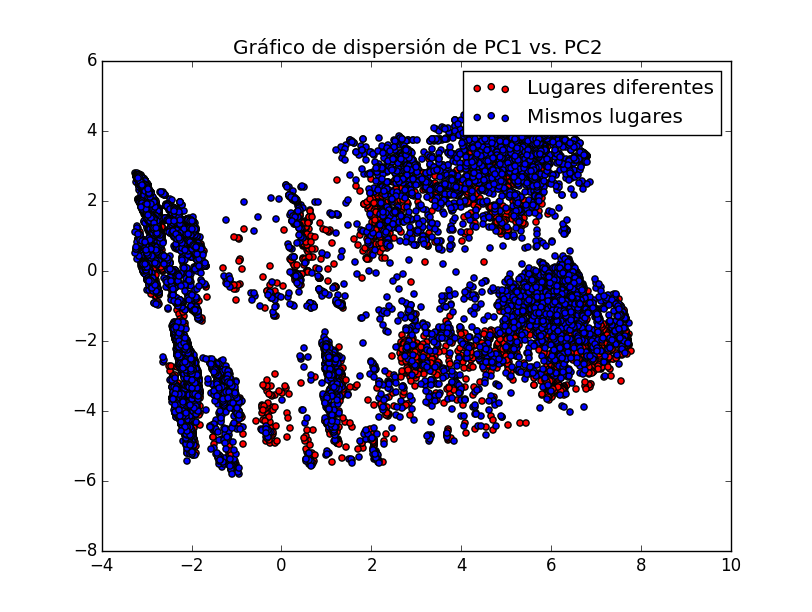
\includegraphics[width=10cm,keepaspectratio]{pca1_vs_pca2.png}
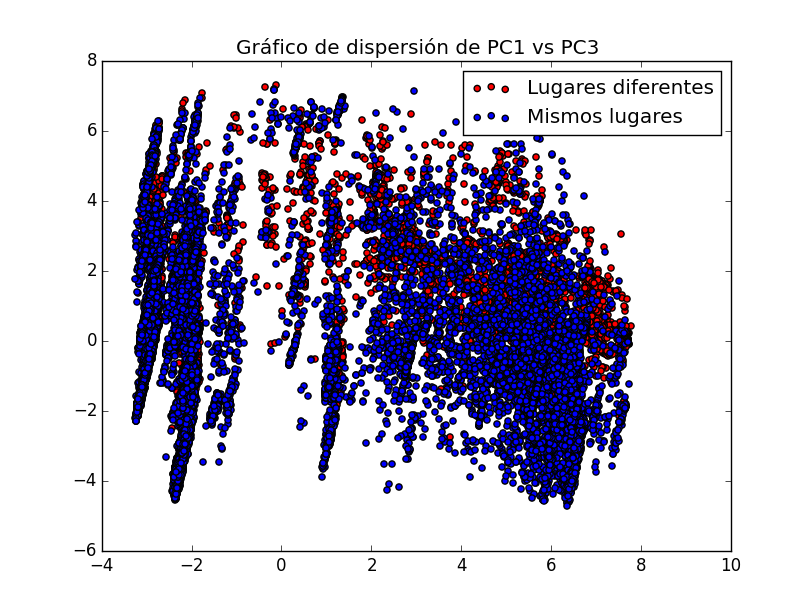
\includegraphics[width=10cm,keepaspectratio]{pca1_vs_pca3.png}
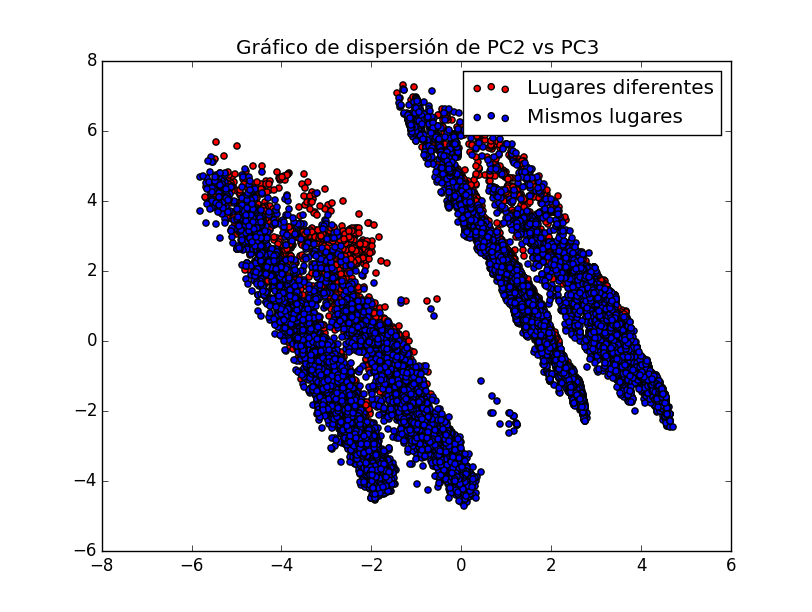
\includegraphics[width=10cm,keepaspectratio]{pca2_vs_pca3.png}
\end{figure}


La tabla \ref{table:main_results} muestra la efectividad en la clasificación
y los tiempos de ejecución de cada uno de los algoritmos descriptos en
la sección de \textit{Materiales}

El ensamble tiene una performance del 97.78\%.

\begin{table}[!hb]
\caption{Performance crossvalidada de todos los clasificadores}
\label{table:main_results}
\centering
\begin{tabular}{l | l l l | l l}
	Id	&	Clasificador	&	Degree	&    $\gamma$	& Tiempo [s]  &	Performance \\
	&			&		&		&	CrossVal.	&	CrossVal. \\
\hline
	1	&	LDA	&		&		&	12	&	\textbf{94.14} \\
\hline
	2	&	QDA	&		&		&	15	&	42.00 \\
\hline
	3	&	SVM lineal 	&		&		&	156	&	94.82 \\
	4	&	SVM rbf  	&		&	1	&	156	&	94.82 \\
	5	&	SVM rbf  	&		&	0	&	154	&	94.82 \\
	6	&	SVM rbf  	&		&	 0,1 	&	155	&	94.82 \\
	7	&	SVM rbf  	&		&	 0,01 	&	155	&	94.82 \\
	8	&	SVM rbf  	&		&	0,0001	&	155	&	94.82 \\
	9	&	SVM rbf  	&		&	 0,0001 	&	156	&	94.82 \\
	10	&	SVM rbf  	&		&	 0,00001 	&	156	&	94.82 \\
	11	&	SVM polinómico 	&	2	&	1	&	774	&	96.06 \\
	12	&	SVM polinómico 	&	2	&	0	&	181	&	94.44 \\
	13	&	SVM polinómico 	&	2	&	 0,1  	&	138	&	96.13 \\
	14	&	SVM polinómico 	&	2	&	 0,01  	&	168	&	95.11 \\
	15	&	SVM polinómico 	&	2	&	0,0001	&	404	&	92.44 \\
	16	&	SVM polinómico 	&	2	&	 0,0001  	&	551	&	71.44 \\
	17	&	SVM polinómico 	&	2	&	 0,00001  	&	487	&	71.44 \\
	18	&	SVM polinómico 	&	3	&	1	&	1369	&	94.57 \\
	19	&	SVM polinómico 	&	3	&	0	&	199	&	94.5 \\
	20	&	SVM polinómico 	&	3	&	 0,1  	&	196	&	\textbf{96.14} \\
	21	&	SVM polinómico 	&	3	&	 0,01  	&	157	&	95.35 \\
	22	&	SVM polinómico 	&	3	&	0,0001	&	524	&	71.44 \\
	23	&	SVM polinómico 	&	3	&	 0,0001  	&	474	&	71.44 \\
	24	&	SVM polinómico 	&	3	&	 0,00001  	&	477	&	71.44 \\
	25	&	SVM polinómico 	&	4	&	1	&	2005	&	93.65 \\
	26	&	SVM polinómico 	&	4	&	0	&	223	&	94.3 \\
	27	&	SVM polinómico 	&	4	&	 0,1  	&	333	&	95.49 \\
	28	&	SVM polinómico 	&	4	&	 0,01  	&	158	&	95.48 \\
	29	&	SVM polinómico 	&	4	&	0,0001	&	549	&	71.44 \\
	30	&	SVM polinómico 	&	4	&	 0,0001  	&	476	&	71.44 \\
	31	&	SVM polinómico 	&	4	&	 0,00001  	&	475	&	71.44 \\
	32	&	SVM polinómico 	&	5	&	1	&	2251	&	93.42 \\
	33	&	SVM polinómico 	&	5	&	0	&	252	&	94.05 \\
	34	&	SVM polinómico 	&	5	&	 0,1  	&	450	&	94.99 \\
	35	&	SVM polinómico 	&	5	&	 0,01  	&	150	&	95.56 \\
	36	&	SVM polinómico 	&	5	&	0,0001	&	530	&	71.44 \\
	37	&	SVM polinómico 	&	5	&	 0,0001  	&	476	&	71.44 \\
	38	&	SVM polinómico 	&	5	&	 0,00001  	&	473	&	71.44 \\
	39	&	SVM sigmoide 	&		&	1	&	666	&	60.89 \\
	40	&	SVM sigmoide 	&		&	0	&	451	&	71.44 \\
	41	&	SVM sigmoide 	&		&	 0,1 	&	787	&	60.76 \\
	42	&	SVM sigmoide 	&		&	 0,01 	&	446	&	72.39 \\
	43	&	SVM sigmoide 	&		&	0,001	&	270	&	92.92 \\
	44	&	SVM sigmoide 	&		&	 0,0001 	&	436	&	90.94 \\
	45	&	SVM sigmoide 	&		&	 0,00001 	&	550	&	71.44 \\
\hline
	46	&	K-nn	&	3	&		&	68	&	\textbf{94.99} \\
	47	&	K-nn	&	4	&		&	68	&	94.61 \\
	48	&	K-nn	&	5	&		&	71	&	94.81 \\
	49	&	K-nn	&	6	&		&	70	&	94.58 \\
	50	&	K-nn	&	7	&		&	73	&	94.63 \\
	51	&	K-nn	&	8	&		&	74	&	94.5 \\
	52	&	K-nn	&	9	&		&	72	&	94.66 \\
	53	&	K-nn	&	10	&		&	74	&	94.53 \\
	54	&	K-nn	&	11	&		&	75	&	94.48 \\
	55	&	K-nn	&	12	&		&	76	&	94.28 \\
	56	&	K-nn	&	13	&		&	73	&	94.22 \\
	57	&	K-nn	&	14	&		&	76	&	94.1 \\
	58	&	K-nn	&	15	&		&	78	&	94.04 \\
	59	&	K-nn	&	16	&		&	74	&	93.9 \\
	60	&	K-nn	&	17	&		&	74	&	93.97 \\
	61	&	K-nn	&	18	&		&	78	&	93.83 \\
	62	&	K-nn	&	19	&		&	79	&	93.86 \\
	63	&	K-nn	&	20	&		&	75	&	93.78 \\
\end{tabular}
\end{table}


\section{Discusión}
\subsection{Análisis de Componentes Principales}
La tabla \ref{table:pca_results} muestra la varianza acumulada de las
primeras 30 componentes principales. La tabla muestra que el 95\%
de la varianza puede ser explicada con 17 componentes de las 118 variables
totales del dataset. Con 30 componentes principales, se puede explicar
el 99\% de la varianza.

Los gráficos de la figura \ref{fig:pca_scatterplot} muestran 3 scratterplot de
las 3 primeras componentes principales. Los gráficos de la componente principal 1 
contra la componente 2 y 3, muestran que no se pueden identificar las clases, ya
que ambas estan distribuidas por todo el gráfico. En el gráfico de la
componente principal 2 y la 3 ya se puede ver que las clases que apuntan
a \textit{``distintos destinos''}, se encuentran más agrupadas que en las componentes
previas. Sin embargo, pese al mayor poder de agrupamiento, estan muy juntas a
las instancias de la clase contraria, haciendo imposible una clara identificación por
componentes principales.

\subsection{Métodos de clasificación}
El objetivo que se persigue en este trabajo es encontrar varios clasificadores
de diferentes tipos, que tengan una buen desempeño encontrando las clases:
instancias que apuntan al mismo lugar y las que no. El objetivo final es apalancar
el desempeño de estos clasificadores individuales haciendo un ensamble
de los mejores de estos. 
Para esto se prueba distintos tipos de clasificadores con distintos parámetros.
Se prueba con discriminantes lineal de Fisher, discriminante cuadrático,
máquinas de vector soporte y K vecinos mas cercanos. Se intenta en primera 
instancia encontrar el mejor clasificador de cada tipo. Luego, se verifica si
haciendo un ensamble de los mejores, la performance general es aún mejor.

Se aclara que todas las mediciones de performance en esta
sección son aplicando cross-validation, a excepción de que se mencione lo
contrario.

\subsection{Análisis discriminante lineal y cuadrático de Fisher}
El análisis de discriminantes lineal y cuadrático son los únicos de los probados
que no requieren una combinación de parámetros para escoger el mejor. El
clasificador por discriminantes de Fisher lineal pudo diferenciar correctamente
el 94,14\% de las instancias. Es curioso que el clasificador cuadrático tiene
una performace 42,00\%, por debajo del clasificador lineal y más aún, por debajo
del azar. 

Dado estos resultados, se opta por seleccionar el clasificar lineal de Fisher
para ser usado en el ensamble.

\subsection{Máquinas de vector soporte}
Las máquinas de vector soporte son buenas clasificadoras para algunos problemas complejos, permiten
clasificar datos no lineales y en algunos casos tienen una perforance superior a la media.
Como contrapartida, son costosas de entrenar: consumen mucha  memoria y
demandan muchas operaciones de CPU, y además hay que encontrar
los parámetros empíricos que mejor se ajustan a los datos.  
Se intenta escoger el mejor modelo de maquinas de vector soporte. Se
decide probar con 4 kernels distintos y combinar parámetros sobre
cada uno de ellos, para escoger finalmente un modelo para formar parte
del ensamble definitivo. Se prueban 4 kerners: lineal, RBF, polinómico y
sigmoide. El modelo lineal, el más estándar de todos y usado como referencia,
puede clasificar correctamente el 94.82\% de los datos. El modelo RBF, para
sorpresa del autor, tiene exactamente el mismo desempeño que el lineal, 
en cualquier de sus variantes. Por este motivo se descarta este modelo,
ya que es uno más complejo sin valor agregado. 

Respecto al kernel polinómico se prueba con grado 2, 3, 4 y 5. A cada
uno de ellos se los corre con varios valores de $\gamma$ (entre 1 y $10^{-5}$) . Los modelos
con buen desempeño tienen una performance que oscilan entre el 92 y
96\%. Para todos los grados el mejor $\gamma$ es de 0.1, excepto para el polinómico
de grado 5, cuyo mejor $\gamma$ es de 0.01. 

Si se considera el mejor $\gamma$ de cada kernel polinómico, todos los modelos tienen un
desempeño de entre el 95\% y 96\%.

Respecto a los tiempos de ejecución, estos crecen sensiblemente a medida que el $\gamma$ 
disminuye. Esto se debe a que mientras menor es el $\gamma$, mayor es la precisión que 
se le exige al modelo y mas cálculos aritméticos hay que realizar para encontrar
el polinomio discriminante. 

Respecto al kernel sigmoide, solo se obtiene buenos resultados con $\gamma$ iguales
a 0.001 y 0.0001. Para los distintos $\gamma$, la performance era del orden del
70\%.

Tras evaluar los 43 modelos distintos de maquinas de vector soporte, se escoge
la de kernel polinómico de grado 3 y $\gamma=0.1$ porque tiene una performance del
96.14\%, siendo esta la mejor de todas.

\subsection{K vecinos mas cercanos}
Se realizan corridas de K vecinos más cercanos, iterando con K desde
3 a 20 y distancia de Minkowski. En todos los casos se clasificaron
correctamente entre el 93\% y 95\% de las instancias. Los tiempos de corrida aumentaron
a medida que K aumentaba, pero siempre estos tiempos son sensiblemente
mas bajos que los de máquinas de vector soporte.

Lo curioso de este clasificador es que para este problema puntual, a medida
que aumenta el K, disminuye la capacidad de predicción. De cualquier modo,
se debe tener en cuenta que esta diferencia no es mayor a 1.20\%.

Se escoge el clasificador con K=3 para ser usado en el ensemble final,
porque su performance del 94.99\% es la mayor de esta especie.

\subsection{Ensemble}
La tabla \ref{table:ensemble_summary} resume los 3 clasificadores usados 
como base para el ensamble. El ensamble construido es por votos, lo que
significa que la clase seleccionada es la escogida por 2 de los
3 clasificadores.

\begin{table}[ht!]
\caption{Clasificadores individuales y ensemble}
\label{table:ensemble_summary}
\centering
\begin{tabular}{l | l l l }
Tipo & Performance  \\
\hline
LDA & 94.14 \\
SVM polinómico & 96.14 \\
K-nn & 94.99 \\
\hline
\textbf{Ensemble} & \textbf{97.78} \\
\end{tabular}
\end{table}

La performance del ensamble es de un 97.78\%, superior a todos los
clasificadores individuales. Es importante aclarar
que esta es la única medición que no es crossvalidada, sino que el 
procedimiento es separando una muestra de un 20\% para testing y
entrenando nuevamente los 3 clasificadores del ensamble con el 80\%
de entrenamiento.

Se ha intentado mejorar la performance usando mas clasificadores de
máquinas vector soporte o K vecinos mas cercanos, obteniendo los
mismos resultados. Es por esto que se escoge usar el ensemble
mas simple como clasificador del desafío planteado.


\section{Conclusiones}
Se ha logrado construir un ensemble de clasificadores capaz de identificar
con un 97.78\% si 2 registros de ubicaciones pertenecen al mismo destino o no,
usando los datos transformados y provistos por el motor de búsqueda de Nomao.



\appendices

\section{Especificación de los datos provistos por Nomao}
\label{appendix1}
Todas las variables categóricas pueden tener 3 valores posibles:
\textit{'n'}, \textit{'s'} o \textit{'m'}.
Todas las variables continuas son reales con valores entre 
0 y 1. Las variables continuas pueden tener valores faltantes.

\begin{table}[ht!]
\caption{Descripción de las 118 variables} 
\label{table:data_set}
\begin{tabular}{l | l l }
Numero & Nombre & Tipo \\
       &        &      \\
\hline
1	& id  & string  \\
2	& clean\_name\_intersect\_min  &   real  \\
3	& clean\_name\_intersect\_max  &   real  \\
4	& clean\_name\_levenshtein\_sim  &   real  \\
5	& clean\_name\_trigram\_sim  &   real  \\
6	& clean\_name\_levenshtein\_term  &   real  \\
7	& clean\_name\_trigram\_term  &   real  \\
8	& clean\_name\_including  &    categorica   \\
9	& clean\_name\_equality  &    categorica   \\
10	& city\_intersect\_min  &   real  \\
11	& city\_intersect\_max  &   real \\
12	& city\_levenshtein\_sim  &   real  \\
13	& city\_trigram\_sim  &   real  \\
14	& city\_levenshtein\_term  &   real  \\
15	& city\_trigram\_term  &   real  \\
16	& city\_including  &    categorica   \\
17	& city\_equality  &    categorica   \\
18	& zip\_intersect\_min  &   real  \\
19	& zip\_intersect\_max  &   real  \\
20	& zip\_levenshtein\_sim  &   real  \\
21	& zip\_trigram\_sim  &   real  \\
22	& zip\_levenshtein\_term  &   real  \\
23	& zip\_trigram\_term  &   real  \\
24	& zip\_including  &    categorica   \\
25	& zip\_equality  &    categorica   \\
26	& street\_intersect\_min  &   real  \\
27	& street\_intersect\_max  &   real  \\
28	& street\_levenshtein\_sim  &   real  \\
29	& street\_trigram\_sim  &   real  \\
30	& street\_levenshtein\_term  &   real  \\
31	& street\_trigram\_term  &   real  \\
32	& street\_including  &    categorica   \\
33	& street\_equality  &    categorica   \\
34	& website\_intersect\_min  &   real  \\
35	& website\_intersect\_max  &   real  \\
36	& website\_levenshtein\_sim  &   real  \\
37	& website\_trigram\_sim  &   real  \\
38	& website\_levenshtein\_term  &   real  \\
39	& website\_trigram\_term  &   real  \\
40	& website\_including  &    categorica   \\
41	& website\_equality  &    categorica   \\
42	& countryname\_intersect\_min  &   real  \\
43	& countryname\_intersect\_max  &   real  \\
44	& countryname\_levenshtein\_sim  &   real  \\
45	& countryname\_trigram\_sim  &   real  \\
46	& countryname\_levenshtein\_term  &   real  \\
47	& countryname\_trigram\_term  &   real  \\
48	& countryname\_including  &    categorica   \\
49	& countryname\_equality  &    categorica   \\
50	& geocoderlocalityname\_intersect\_min  &   real  \\
51	& geocoderlocalityname\_intersect\_max  &   real  \\
52	& geocoderlocalityname\_levenshtein\_sim  &   real  \\
53	& geocoderlocalityname\_trigram\_sim  &   real  \\
54	& geocoderlocalityname\_levenshtein\_term  &   real  \\
55	& geocoderlocalityname\_trigram\_term  &   real  \\
56	& geocoderlocalityname\_including  &    categorica   \\
57	& geocoderlocalityname\_equality  &    categorica   \\
58	& geocoderinputaddress\_intersect\_min  &   real  \\
59	& geocoderinputaddress\_intersect\_max  &   real  \\
60	& geocoderinputaddress\_levenshtein\_sim  &   real  \\
61	& geocoderinputaddress\_trigram\_sim  &   real  \\
62	& geocoderinputaddress\_levenshtein\_term  &   real  \\
63	& geocoderinputaddress\_trigram\_term  &   real  \\
64	& geocoderinputaddress\_including  &    categorica   \\
65	& geocoderinputaddress\_equality  &    categorica   \\
66	& geocoderoutputaddress\_intersect\_min  &   real  \\
67	& geocoderoutputaddress\_intersect\_max  &   real  \\
68	& geocoderoutputaddress\_levenshtein\_sim  &   real  \\
69	& geocoderoutputaddress\_trigram\_sim  &   real  \\
70	& geocoderoutputaddress\_levenshtein\_term  &   real  \\
\end{tabular}
\end{table}

\begin{table}[ht!]
\centering
\begin{tabular}{l | l l l}
Numero & Nombre & Tipo & Rango \\
       &        &      &                 \\
\hline
71	& geocoderoutputaddress\_trigram\_term  &   real  \\
72	& geocoderoutputaddress\_including  &    categorica   \\
73	& geocoderoutputaddress\_equality  &    categorica   \\
74	& geocoderpostalcodenumber\_intersect\_min  &   real  \\
75	& geocoderpostalcodenumber\_intersect\_max  &   real  \\
76	& geocoderpostalcodenumber\_levenshtein\_sim  &   real  \\
77	& geocoderpostalcodenumber\_trigram\_sim  &   real  \\
78	& geocoderpostalcodenumber\_levenshtein\_term  &   real  \\
79	& geocoderpostalcodenumber\_trigram\_term  &   real  \\
80	& geocoderpostalcodenumber\_including  &    categorica   \\
81	& geocoderpostalcodenumber\_equality  &    categorica   \\
82	& geocodercountrynamecode\_intersect\_min  &   real  \\
83	& geocodercountrynamecode\_intersect\_max  &   real  \\
84	& geocodercountrynamecode\_levenshtein\_sim  &   real  \\
85	& geocodercountrynamecode\_trigram\_sim  &   real  \\
86	& geocodercountrynamecode\_levenshtein\_term  &   real  \\
87	& geocodercountrynamecode\_trigram\_term  &   real  \\
88	& geocodercountrynamecode\_including  &    categorica   \\
89	& geocodercountrynamecode\_equality  &    categorica   \\
90	& phone\_diff  &   real  \\
91	& phone\_levenshtein  &   real  \\
92	& phone\_trigram  &   real  \\
93	& phone\_equality  &    categorica   \\
94	& fax\_diff  &   real  \\
95	& fax\_levenshtein  &   real  \\
96	& fax\_trigram  &   real  \\
97	& fax\_equality  &    categorica   \\
98	& street\_number\_diff  &   real  \\
99	& street\_number\_levenshtein  &   real  \\
100	& street\_number\_trigram  &   real  \\
101	& street\_number\_equality  &    categorica   \\
102	& geocode\_coordinates\_long\_diff  &   real  \\
103	& geocode\_coordinates\_long\_levenshtein  &   real  \\
104	& geocode\_coordinates\_long\_trigram  &   real  \\
105	& geocode\_coordinates\_long\_equality  &    categorica   \\
106	& geocode\_coordinates\_lat\_diff  &   real  \\
107	& geocode\_coordinates\_lat\_levenshtein  &   real  \\
108	& geocode\_coordinates\_lat\_trigram  &   real  \\
109	& geocode\_coordinates\_lat\_equality  &    categorica   \\
110	& coordinates\_long\_diff  &   real  \\
111	& coordinates\_long\_levenshtein  &   real  \\
112	& coordinates\_long\_trigram  &   real  \\
113	& coordinates\_long\_equality  &    categorica   \\
114	& coordinates\_lat\_diff  &   real  \\
115	& coordinates\_lat\_levenshtein  &   real  \\
116	& coordinates\_lat\_trigram  &   real  \\
117	& coordinates\_lat\_equality  &    categorica   \\
118	& geocode\_coordinates\_diff  &   real  \\
119	& coordinates\_diff  &   real  \\
120	& label (clase) & categorica (1 o 0). \\
\end{tabular}
\end{table}



\end{document}

